\begin{center}
    \addcontentsline{toc}{section}{ГЛАВА 2. SLAM-АЛГАРЫТМЫ}
    \section*{ГЛАВА 2. \\ SLAM-АЛГАРЫТМЫ}
\end{center}

\addcontentsline{toc}{subsection}{2.1 Агляд}
\subsection*{2.1 Агляд}

Задача адначасовай лакалізацыі і пошуку на мапе (Simultaneous Localization and Mapping, SLAM)
спалучае ў сабе выкарыстанне разнастайных датчыкаў (лазерныя сканеры, RGB альбо RGB-D
камеры і гэтак далей) з мэтай ацэнкі пазіцыі ў прасторы і адначасовай пабудовы мапы мясцовасці.
Задача фармулюецца як для двухмерных, так і для трохмерных асяроддзяў: нас больш цікавіць
трохмерная задача, тым больш што двухмерная версія задачы лічыцца вырашанай. З адначасовасці
пабудовы мапы і ацэнкі пазіцыі ў прасторы вынікае патрэбнасць да алгарытма працаваць у рэальным часе,
што накладае асаблівыя патрабаванні да алгарытмаў і абсталявання, на якім алгарытмы запускаюцца.

Сваё найбольшае развіццё рашэнне SLAM задачы атрымала ў апошнія дзесяцігоддзі. Даследванне
задачы можна ўмоўна падзяліць на тры этапы (прапанаваныя ў \cite{DBLP:journals/corr/CadenaCCLSN0L16},
\cite{Li2016RealtimeSL}). Першы перыяд, прыблізна 1986-2004, можна назваць ``класічным''.
У гэтыя часы асноўным накірункам працы па рашэнні задачы была імавернасная фармуліроўка
і падыходы, заснаваныя на фільтрах. У другі перыяд, 2004-2015, былі даследаваныя асноўныя
ўласцівасці і падыходы, такія як збежнасць і ўзгодненасць алгарытмаў. У гэты час былі
праведзеныя цесныя аналогія з існуючымі падыходамі ў галіне кампутарнага зроку.

Мяркуюцца, што на трэці этап распрацоўка перайшла зусім нядаўна, у апошнія гады: гэта звязваюць
з публікацыямі такіх алгарытмаў, як, напрыклад, ORB-SLAM альбо LSD-SLAM, якія па сваёй
функцыянальнасці моцна пераўзыходзяць любыя ранейшыя публікацыі. Прынцып працы гэтых алгарытмаў
будзе разгледжаны далей.

Важна успрымаць SLAM не як адзін суцэльны алгарытм, але як канцэпт. SLAM складаецца са
шматлікіх этапаў і кожны з гэтых этапаў можа вырашацца рознымі алгарытмамі з той ці іншай эфектыўнасцю.

Для задачы рэканструкцыі паверхні SLAM-сістэма наўрад ці будзе
аптымальным рашэннем: пабудова шчыльных мадэляў у рэальным часе пакуль яшчэ застаецца
слаба вырашанай задачай. Тут і далей SLAM-сістэмы нас цікавяць сваімі выходнымі
дадзенымі: пасля апрацоўкі дадзеных у рэальным часе захаваныя пазіцыі і павароты камер
у часе і пабудаваная глабальная мапа могуць быць эфектыўна выкарыстаныя ў якасці
ўваходных дадзеных афлайн алгарытма, падвышаючы ягоную дасканальсць і хуткасць працы.

Як вынікае з назвы, алгарытмы рашаюць дзве асноўныя задачы: лакалізацыю і пошук на мапе.
На першых этапах даследвання задачы разглядаліся асобна, але з цягам часу стала зразумела,
што задачы цесна звязаныя і рашэнне адной з іх моцна дапамагае ў рашэнні іншай. Мапа патрэбная для
эфектыўнага пошуку пазіцыі ў прасторы, у той жа час з ацэнкай становішча мапа сабірае больш дадзеных
і становіцца больш дакладнай. Асобнай задачай заўжды стаіць магчымасць алгарытма
замыкаць цыклы (\textit{loop closure}).

Разгледзім асноўныя этапы падрабязней.

\addcontentsline{toc}{subsubsection}{2.1.1 Лакалізацыя}
\subsubsection*{2.1.1 Лакалізацыя}

Пры руху пазіцыя БПЛА ў дыскрэтным часе задаецца матрыцай $T \in \mathbb{R}^{4\times4}$.
Паслядоўнасць такіх матрыцаў - траекторыя пралёту. Лакалізацыя - пошук такой матрыцы ў вызначаны момант часу.
Для адкрытых прастораў задача была часткова вырашаная з запускам GPS - глабальнай сістэмы
пазіцыянавання; у прасторах, дзе GPS недаступны, таксама можа выкарыстоўвацца вонкавае
абсталявання для лакалізацыі, што часта з'яўляецца непрактычным альбо дарагім рашэннем.
Выкарыстанне датчыкаў, усталяваных на БПЛА, для лакалізацыі ў прасторы, робіць падыходы
да рашэння задачы больш універсальнымі. Лакалізацыю з дапамогай толькі камераў часам
таксама называюць візуальнай адаметрыяй (\textit{Visual Odometry}). Надзейныя механізмы
лакалізацыі аўтаномных БПЛА асабліва важныя праз знаходжанне БПЛА ў паветры і
немагчымасць спыніцца, у адрозненні на наземных робатаў.

\addcontentsline{toc}{subsubsection}{2.1.2 Пошук на мапе}
\subsubsection*{2.1.2 Пошук на мапе}

Ёсць некалькі важных аспектаў пабудовы мапы. Па-першае, мапа выкарыстоўваецца для пракладкі
маршрутаў і лакалізацыю перашкодаў - асноўныя элементы для аўтаномнай навігацыі. Па-другое -
мапа на выхадзе можа быць цікавая сама па сабе. Яна можа пасля выкарыстоўвацца для візуалізацыі пралёта
па мясцовасці альбо як уваходныя дадзеныя для алгарытмаў афлайн-рэканструкцыі, для распазнавання
аб'етаў і гэтак далей. Трэці і, магчыма, самы важны аспект у дачыненні да канцэпцыі SLAM -
добра пабудаваная мапа дазваляе лакалізаваць БПЛА ў прасторы.

Такім чынам, лакалізацыя і пошук на мапе не выступаюць як дзве асобныя і незалежныя
часткі алгарытма, але дапаўняюць і паляпшаюць адно аднаго. Пошук сябе на папярэдне пабудаванай мапе
(напрыклад, пры паўторным пралёце той жа мясцовасці) дазваляе лакалізаваць БПЛА з
якасцю параўнальнай з якасцю пабудаванай мапы, у сваю чаргу лакалізацыя пры дапамозе
адаметрыі і старонніх датчыкаў паслядоўна ўдасканальвае мапу.

\addcontentsline{toc}{subsection}{2.2 Падыходы да рэалізацыі}
\subsection*{2.2 Падыходы да рэалізацыі}

Як зазначаецца ў \cite{Li2016RealtimeSL}, архітэктура любой SLAM-сістэмы
можа быць прадстаўленая схемай як на малюнку \ref{fig:slam-architecture}. Фронтэнд выконвае
першасную апрацоўку дадзеных, якія паступаюць са знешніх датчыкаў. Для алгарытмаў,
заснаваных на пошуку асаблівых кропак, фронтэнд займаецца іх пошукам і апісаннем;
для алгарытмаў, якія працуюць непасрэдна са значэннямі пікселяў, выконваецца трэкінг паміж
кадрамі. Усе вынікі першаснай апрацоўкі пасля перадаюцца бэкэнду.

Бэкэнд, у сваю чаргу, займаецца пабудовай графа залежнасцяў, аптымізацыяй на графе.

Важным крокам у рэалізацыя SLAM-алгарытмаў стала дамінаванне ідэі раздзялення лакалізацыі
і пошуку на мапе ў асобныя плыні. Упершыню практычнае прымяненне ідэя знайшла
ў сістэме PTAM (\textit{Parallel Tracking and Mapping for Small AR Workspaces}, \cite{Klein:2007:PTM:1514339.1514363}).
Лакалізацыйная плыня PTAM займаецца пошукам адпаведнасцяў у дадзеных і запускае
аптымізацыю па рухах камеры. У гэты ж час плыня з мапай калекцыянуе вынікі лакалізацыі,
трыангулюе выяўленыя асаблівасці ў трохмерныя кропкі і абнаўляе глабальную мапу.
Са з'яўленнем такога падыходу сталі відавочнымі ягоныя перавагі і амаль кожная
сучасная SLAM-сістэма пабудаваная па падобным прынцыпе.

\begin{figure}[H]
  \centering
  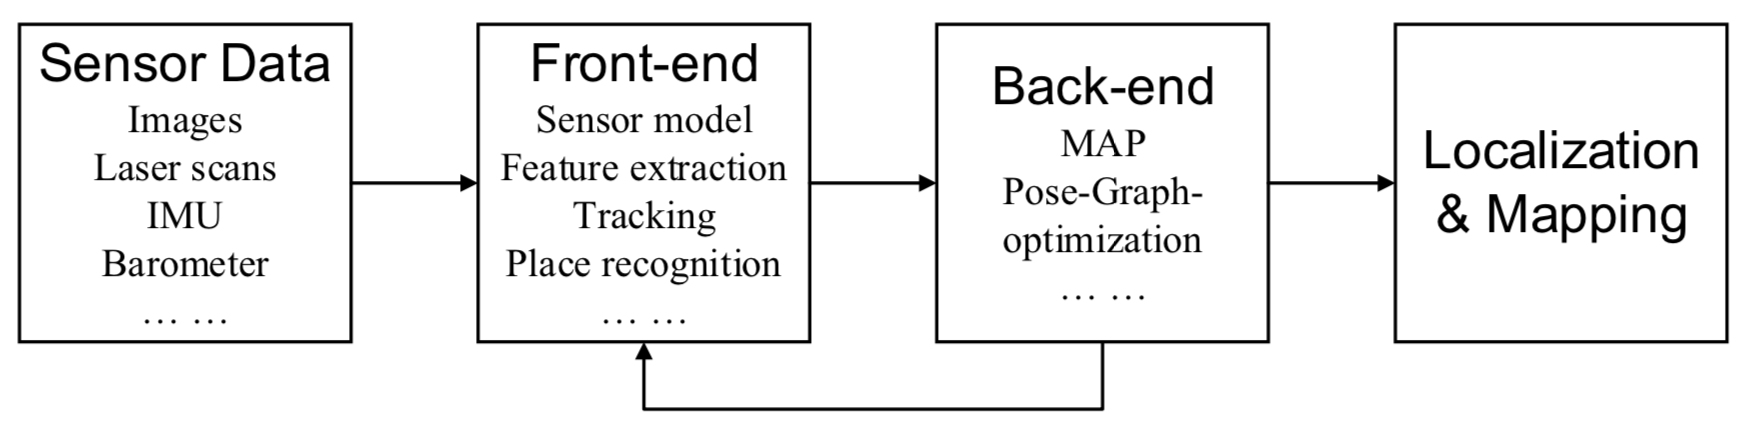
\includegraphics[width=.9\textwidth]{slam-architecture}
  \captionsetup{labelformat=empty}
  \caption{Малюнак \arabic{figure}: архітэктура SLAM-алгарытмаў}
  \label{fig:slam-architecture}
\end{figure}

\addcontentsline{toc}{subsection}{2.3 Агляд SLAM-рэалізацыяў}
\subsection*{2.3 Агляд SLAM-рэалізацыяў}

Далей ідзе апісанне асаблівасцяў некалькі SLAM-сістэм, якія паказваюць найлепшыя вынікі.
Адна з іх заснаваныя на пошуку асаблівых кропак (\textit{feature-based SLAM}),
другая - на простых метадах (\textit{direct SLAM}), трэцяе - камбінуе ў сабе
абодва падыхода (\textit{semi-direct SLAM}).

\addcontentsline{toc}{subsubsection}{2.3.1 ORB-SLAM}
\subsubsection*{2.3.1 ORB-SLAM}

ORB-SLAM (\cite{murTRO2015}, \cite{murORB2}) - манакулярная SLAM-сістэма,
заснаваная на пошуку асаблівасцяў на выявах (\textit{feature-based}),
спраектаваная для працы ў маленькіх і вялікіх, замкнёных і адкрытых прасторах.

\begin{figure}[H]
  \centering
  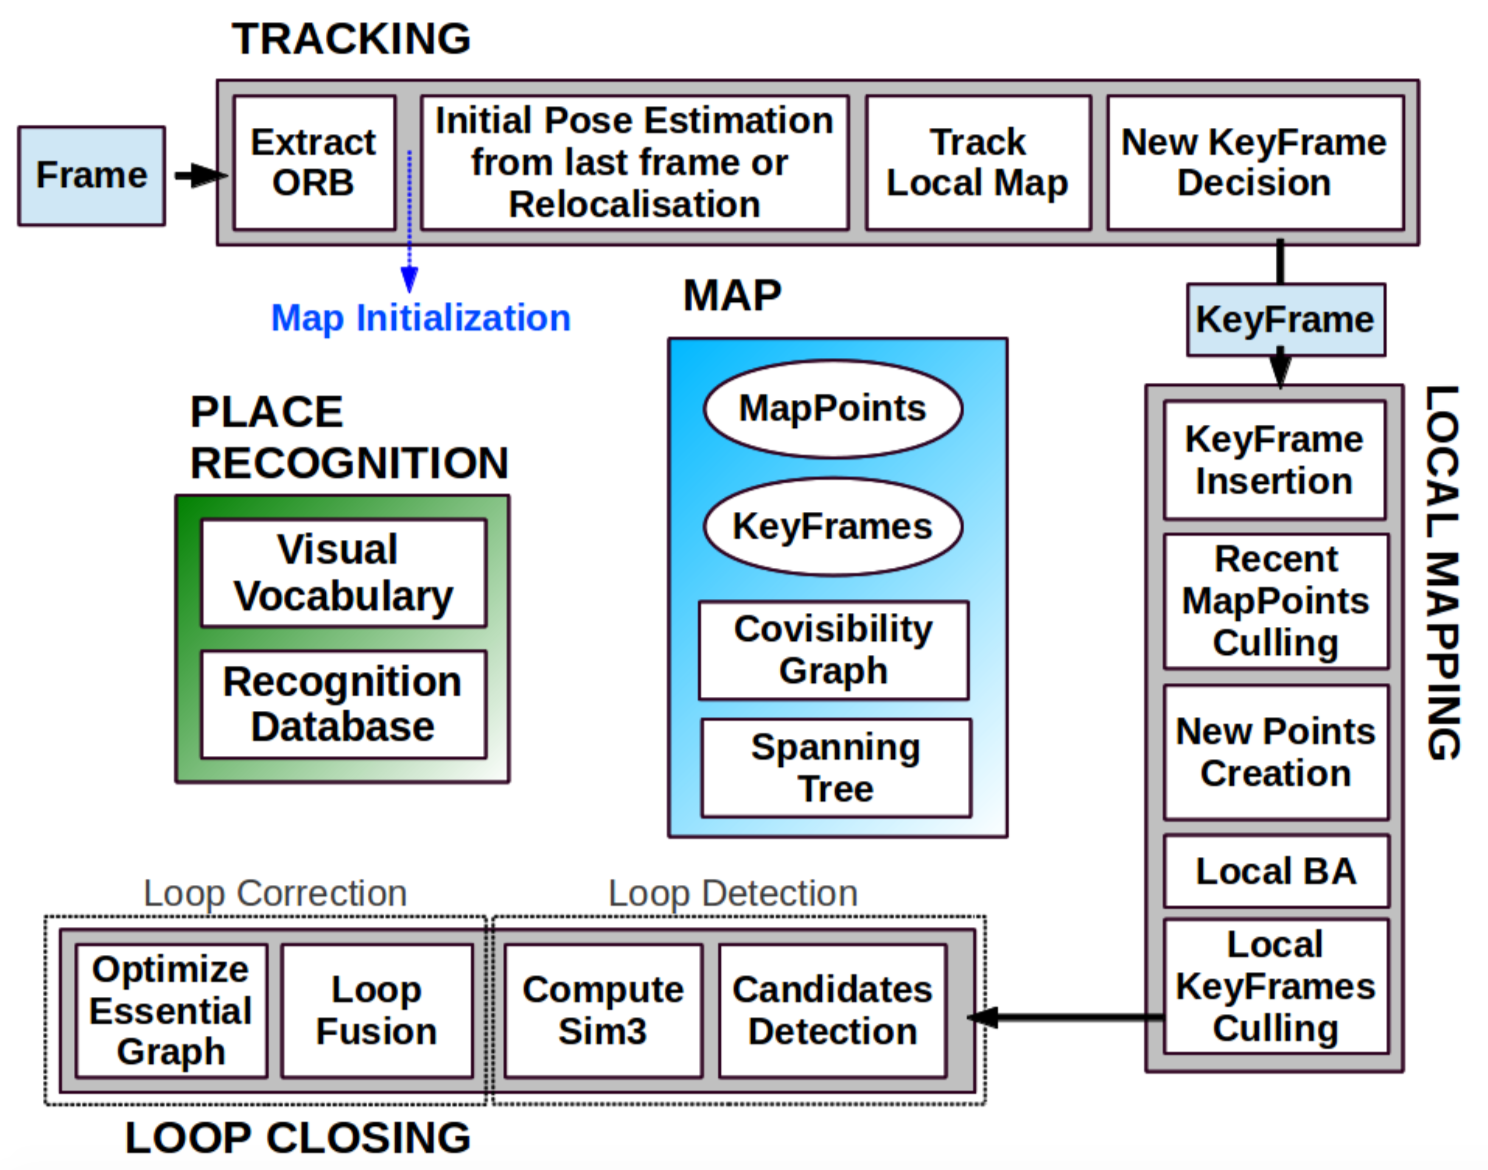
\includegraphics[width=.7\textwidth]{orb-architecture}
  \captionsetup{labelformat=empty}
  \caption{Малюнак \arabic{figure}: ORB-SLAM}
  \label{fig:orb-architecture}
\end{figure}

Асноўныя асаблівасці:

\begin{itemize}
  \item выкарыстанне адных і тых жа ключавых кропак на ўсіх этапах працы алгарытма;
  \item чатыры асноўныя задачы, якія адначасова рашае алгарытм: трэкінг (\textit{tracking}),
  нанясенне дадзеных на мапу (\textit{mapping}), рэлакалізацыя (\textit{relocalization}),
  замкненне цыклаў (\textit{loop closing});
  \item неабмежаваны рост памераў мапы \textit{толькі} з ростам аглядаемай тэрыторыі;
  \item выкарыстанне ORB-дэскрыптараў як найлепшых па хуткасці (без ужывання GPU)
  і інварыянтнасці да зменаў у павароце і асвятленні;
  \item хуткі трэкінг і пошук на мапе на лакальных абласцях бачнасці, што дасягаецца
  праз выкарыстанне \textit{графа бачнасці} (\textit{covisibility graph});
  \item новы аўтаматычны і надзейны спосаб ініцыялізацыі, які стварае пачатковы мапы
  як для планарных, так і непланарных паверхняў;
  \item пазбаўленне ад лішніх ключавых кадраў па стратэгіі ``выжывання наймацнейшага''
  (\textit{survival of the fittest});
  \item агульная схема працы алгарытма прадстаўленая на малюнку \ref{fig:orb-architecture}.
\end{itemize}

Арыгінальная публікацыя \cite{murTRO2015} прыводзіла апісанне манакулярнай сістэмы,
у другой рэдакцыі алгарытма (ORB-SLAM2, \cite{murORB2}) дадалася падтрымка стэрэа і RGB-D камер.
Пра рэалізацыю варта зазначыць, што першая версія была даступная толькі пад ROS,
у сваю чаргу ў другой версіі з'явіўся ўласны візуалізатар, здольны працаваць незалежна.

\addcontentsline{toc}{subsubsection}{2.3.3 LSD-SLAM}
\subsubsection*{2.3.3 LSD-SLAM}

У адрозненні ад разгледжанай вышэй сістэмы ORB-SLAM, заснаванай на пошуку
асаблівых кропак, LSD-SLAM (\cite{engel14eccv}) выкарыстоўвае \textit{простыя} (\textit{direct})
падыходы да працы з выявамі, то бок працуе непасрэдна са значэннямі ў пікселях.

\begin{figure}[H]
  \centering
  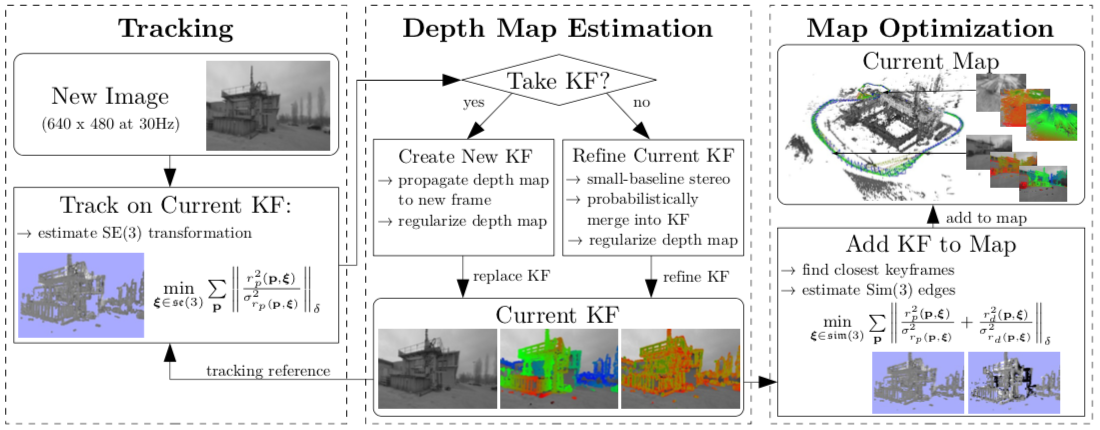
\includegraphics[width=.8\textwidth]{lsd-architecture}
  \captionsetup{labelformat=empty}
  \caption{Малюнак \arabic{figure}: LSD-SLAM}
  \label{fig:lsd-architecture}
\end{figure}

\begin{itemize}
  \item працуе ў рэальным часе на CPU;
  \item складаецца з трох асноўных кампанент: трэкінг, падлік набліжэння для мапы
  глыбіняў і аптымізацыя мапы;
  \item трэкінг кампанента паслядоўна апрацоўвае новыя здымкі, прымаючы да ўвагі
  папярэдні і бягучы ключавы здымкі;
  \item другая кампанента выкарыстоўвае здымкі каб альбо палепшыць, альбо замяніць
  бягучы ключавы кадр і ацэньвае глыбіню сцэны простымі (\textit{direct})
  і імавернаснымі падыходамі;
  \item здымкі, якія канчаткова пазначаныя як ключавыя (мапа глыбіняў больш
  змяняцца не будзе) заносяцца на глабальную мапу;
  \item мапа - граф узаемаразмяшчэнне ключавых кадраў. Паколькі алгарытм таксама
  ацэньвае мапы глыбіняў, то мапа, па сутнасці, ўяўляе сабой напаўшчыльную
  трохмерную рэканструкцыю паверхні;
  \item аўтары ініцыялізуюць першы ключавы кадр \textit{выпадковай} мапай глыбіняў
  з вялікімі перападамі. Сцвярджаецца, што пры значных рухах камеры ў прасторы
  ў першую секунду, першасная мапа глыбіняў будзе хутка збягацца. Аўтары прызнаюцца
  ў неабходнасці дапрацаваць гэтую частку сістэмы; пры тэставых запусках мапа
  глыбіняў для ініцыялізацыі бралася непасрэдна з датасэтаў (то бок была дакладна
  вядомая), на практыцы падобны падыход можа запатрабаваць пэўнага чалавечага ўдзелу;
  \item архітэктура сістэмы прадстаўленая на малюнку \ref{fig:lsd-architecture}.
\end{itemize}

\addcontentsline{toc}{subsubsection}{2.3.2 SVO}
\subsubsection*{2.3.2 SVO}

У адрозненні ад папярэдніх двух прыкладаў, SVO (\textit{Semi-Direct Monocular Visual Odometry},
\cite{Forster2014ICRA}) спалучае ў сабе як пошук і апісанне ключавых кропак, так і
простыя метады.

\begin{figure}[H]
  \centering
  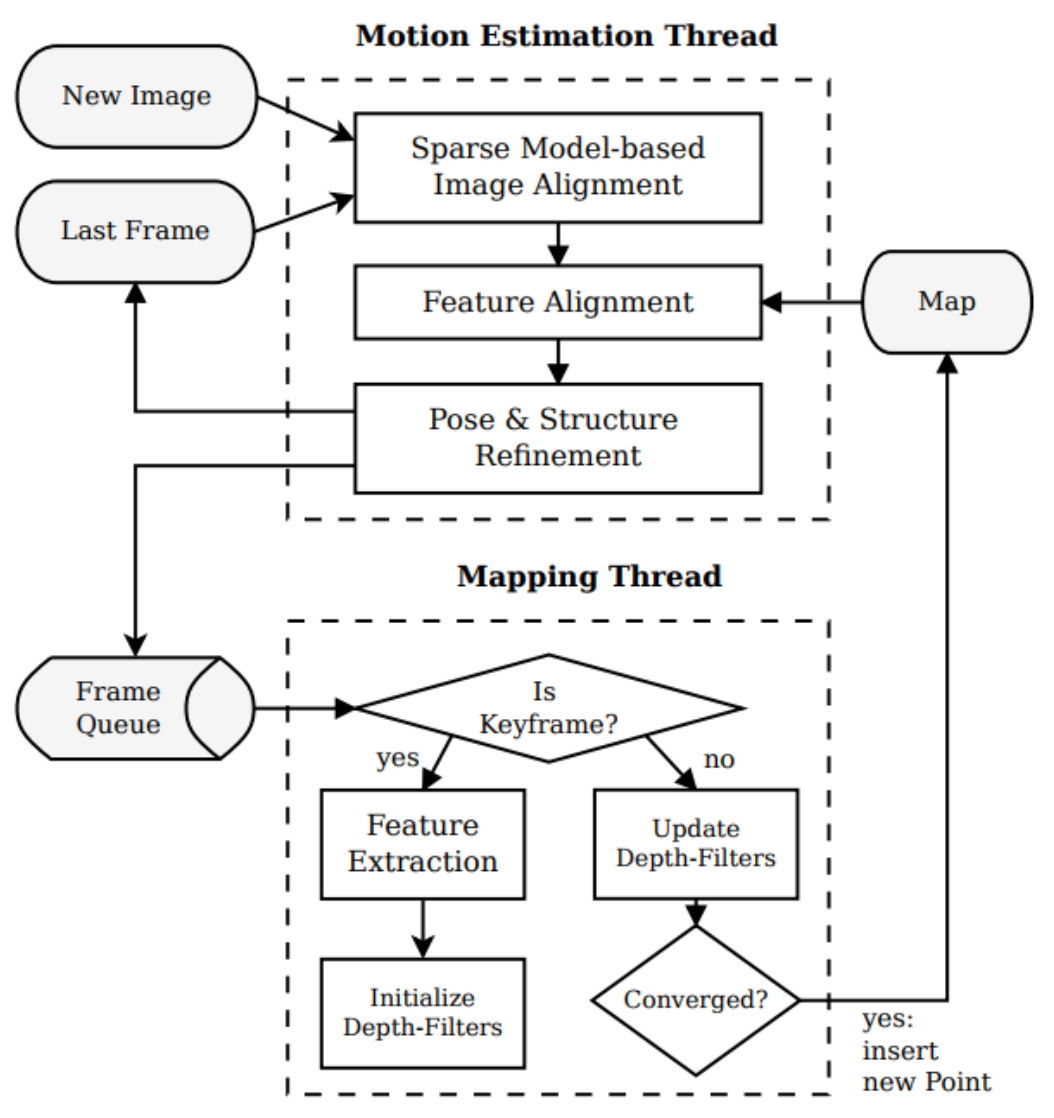
\includegraphics[width=.5\textwidth]{svo-architecture}
  \captionsetup{labelformat=empty}
  \caption{Малюнак \arabic{figure}: SVO}
  \label{fig:svo-architecture}
\end{figure}

\begin{itemize}
  \item спалучае ў сабе лепшае ад метадаў, заснаваных на ключавых кропках (выбар
  ключавых кадраў, сачэнне за мноствам кропак, паралельны трэкінг і пошук на мапе),
  і ад простых метадаў (хуткасць і дакладнасць);
  \item пошук адпаведнасцяў паміж ключавымі кропкамі здзяйсняецца няяўна як вынік
  прымянення простых метадаў (а не matching-а, напрыклад);
  \item выманне ключавых кропак здзяйсняецца толькі на ключавых кадрах;
  \item трохмерная кропка дадаецца на мапу толькі ў выпадку збежнасці адпаведнага
  фільтра глыбіняў, што азначае патрэбнасць у шматлікіх вымярэннях для кожнай асобнай кропкі;
  \item свядзенне да мінімума выбрасаў у вымярэннях;
  \item архітэктура сістэмы прадстаўленая на малюнку \ref{fig:svo-architecture}.
\end{itemize}

\newpage
